\documentclass{article}
% \usepackage{showframe}
\usepackage{siunitx}
\usepackage{booktabs}
\usepackage{graphicx}
\usepackage{amsmath}
\usepackage{mathtools}
\usepackage{minted}
\usepackage{tabularx}
\usepackage{url}
% \usepackage{subfig}
\usemintedstyle{xcode}

% \usepackage{fullpage}

\frenchspacing
% \setlength{\parindent}{0ex}
% \setlength{\parskip}{3 ex plus 2 ex minus 1 ex}

\title{Homework 7}
\author{Josh Bradt}
\date{March 14, 2016}

\begin{document}

\maketitle

I compiled a code using the function shown in Listing~\ref{lst:mmul} to time the matrix-matrix multiplication operation with multiple threads. The compiler was Intel ICC version 15.0.0, and the code was compiled for the HPCC \texttt{intel14} cluster with \texttt{-O2} and \texttt{-qopenmp} when appropriate. I reserved a full node of the cluster by asking for 20 cores on one node with the \texttt{intel14} feature, and then ran the code for several values of $N$ and for 1--20 threads.

\begin{listing}[p]
    \begin{minted}[gobble=8,frame=single]{C}
        #define ind(i,j) (i)*matSize+j

        void matrixMultiply(const double* matA, const double* matB,
                            double* out, const size_t matSize)
        {
          #pragma omp parallel for
          for (size_t i = 0; i < matSize; i++) {
            for (size_t j = 0; j < matSize; j++) {
              double sum = 0;
              for (size_t k = 0; k < matSize; k++) {
                sum += matA[ind(i,k)] * matB[ind(k,j)];
                dummy(matA);
              }
              out[ind(i,j)] = sum;
            }
          }
        }
    \end{minted}
    \caption{Matrix-matrix multiplication function.}
    \label{lst:mmul}
\end{listing}

The results are shown in the figures below and are listed in the attached plain-text data file, delimited with tabs. (There are far too many points to list in a table in this document.)

As a function of the size of the matrix, the data agrees quite well with the model $t\sim(2c+r)N_\text{pts}^3/N_\text{threads}$ as shown in Figure~\ref{fig:dimvtime}. The agreement is better for larger numbers of points, which is sensible since the model assumes the matrices don't fit into cache.

As a function of the number of threads, the performance drops quickly until around $N_\text{threads} = 5$ and then levels off, as shown in Figure~\ref{fig:thvtime}. This is very similar to what we saw in the previous assignment (at least for large matrix dimensions). This probably indicates that the memory bandwidth is beginning to constrain the speed of the calculation as the number of threads increases. In the $N=20$ case, on the other hand, there is not a significant improvement in performance as the number of threads increases. This is likely because the entire $20\times 20$ matrix can fit in cache, so multithreading this case could actually slow it down.

\begin{figure}[p]
    \centering
    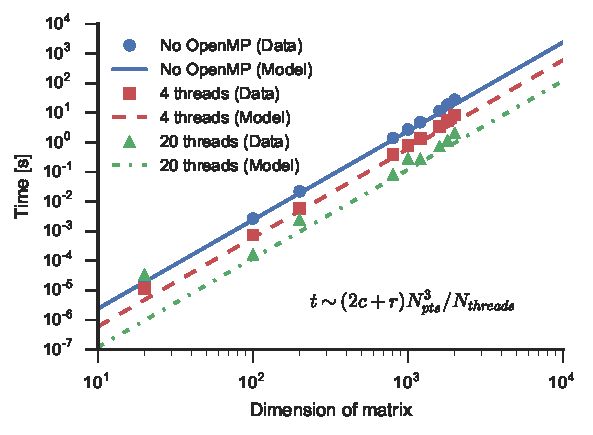
\includegraphics{dim_v_time.pdf}
    \caption{The time taken as a function of the dimension of the matrix, shown in the single-threaded case (blue circles) and for 4 threads and 20 threads (red squares and green triangles, respectively). The lines show the time as calculated by the model $t\sim(2c+r)N_\text{pts}^3/N_\text{threads}$ where $c=1 / (\SI{2.5}{GHz})$ is the time per floating point operation and $r = \SI{1.6}{ns}$ is the time per memory access. These values are taken from the CPU clock frequency and from \textsc{stream}, respectively.}
    \label{fig:dimvtime}
\end{figure}

\begin{figure}[p]
    \centering
    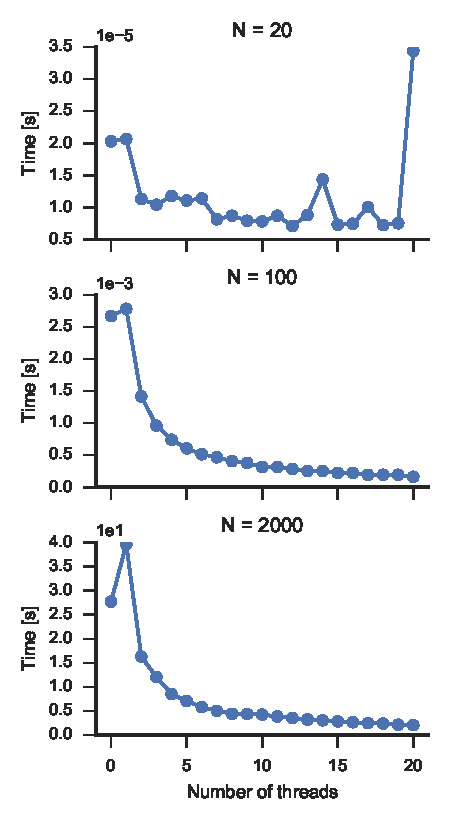
\includegraphics{th_v_time.pdf}
    \caption{The time taken as a function of the number of threads, shown for matrix dimensions $N$ of 20, 100, and 2000. (Note the different scale on each plot, indicated by the multiplier at the top of each vertical axis.) The point with ``0'' threads corresponds to the single-threaded case without OpenMP, while the case with 1 thread corresponds to the code compiled with OpenMP and \texttt{OMP\_NUM\_THREADS=1}.}
    \label{fig:thvtime}
\end{figure}

\begin{figure}[p]
    \centering
    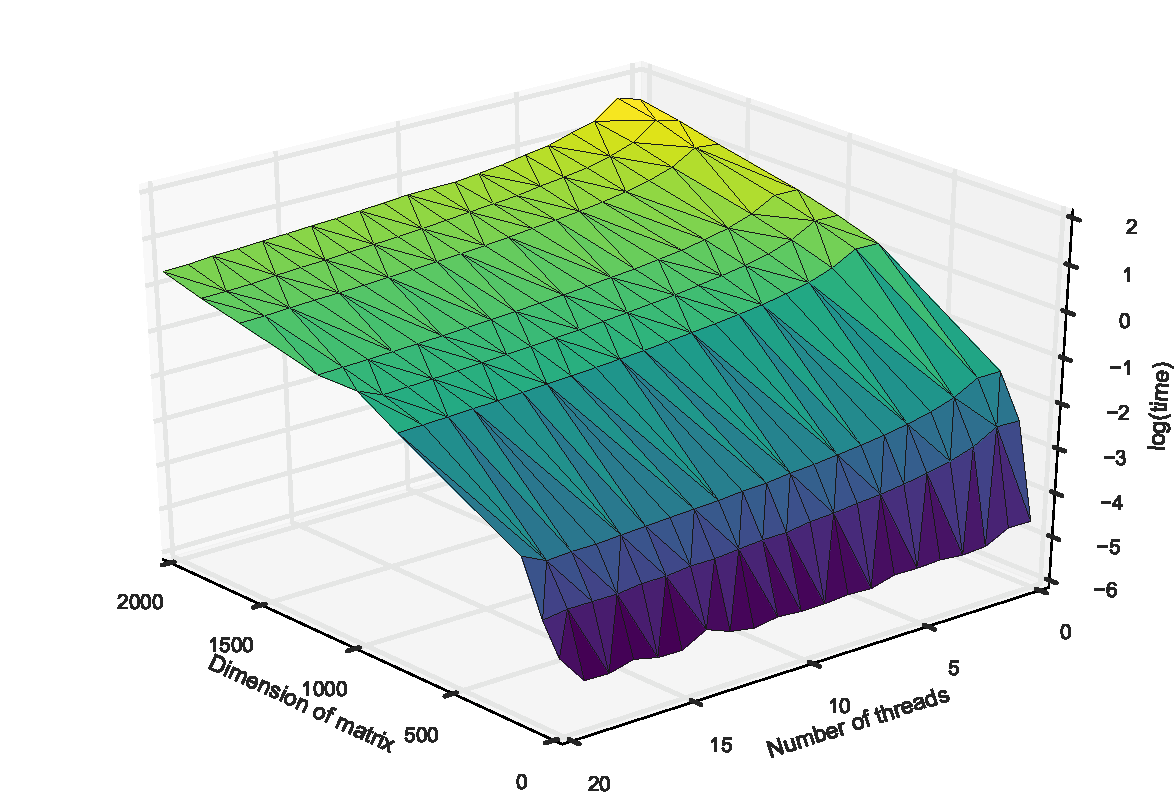
\includegraphics[width=\textwidth]{3d.pdf}
    \caption{Behavior of the time taken as a function of both the dimension of the matrix and the number of threads. The code is the slowest for 1 OpenMP thread and 2000 points, as expected.}
    \label{fig:3d}
\end{figure}


\end{document}
